\documentclass[11pt]{standalone}
\usepackage{amssymb}
\usepackage{amsmath}
\usepackage[no-math]{fontspec}
\usepackage{unicode-math}
\usepackage{libertinus}
\usepackage{pgf,xcolor}
\usepackage{tikz}
\usetikzlibrary{arrows.meta, backgrounds}
\usepackage{pgfplots}
\pgfplotsset{compat=newest}

\definecolor{my_darkgray}{HTML}{484949}
\definecolor{my_lightgray}{HTML}{F3F4F4}
\definecolor{my_darkblue}{HTML}{005A94}
\definecolor{my_lightblue}{HTML}{CCDEE9}
\definecolor{my_yellow}{HTML}{FFEC7F}
\definecolor{my_red}{HTML}{E60000}
\definecolor{my_orange}{HTML}{E87846}

\begin{document}
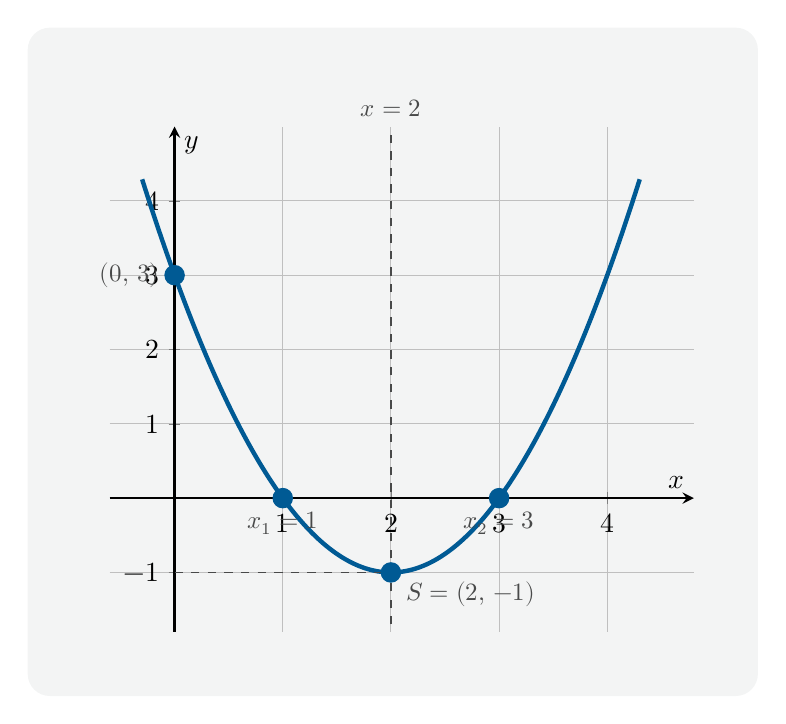
\begin{tikzpicture}[
    show background rectangle,
    background rectangle/.style={fill=my_lightgray, rounded corners=8pt},
    inner frame sep=0.8cm
]
% Parabola: f(x) = x^2 - 4x + 3 = (x-1)(x-3) = (x-2)^2 - 1
% Key features (all used as annotations; no natural-language labels):
%   Vertex:       S = (2, -1)
%   Zeros:        x_1 = 1,  x_2 = 3
%   y-intercept:  (0, 3)
%   Axis of symmetry: x = 2
%   Leading coefficient a = 1 > 0  (opens upward)
\begin{axis}[
    axis lines=center,
    axis line style={thick},
    xlabel={$x$},
    ylabel={$y$},
    height=8cm, width=9cm,
    xmin=-0.6, xmax=4.8,
    ymin=-1.8, ymax=5.0,
    xtick={0,1,2,3,4},
    ytick={-1,0,1,2,3,4},
    grid=both,
    axis line style={thick},
    clip=false,
]

% Axis of symmetry: dashed vertical line at x=2
\draw[dashed, my_darkgray, thick]
    (axis cs:2, -1.7) -- (axis cs:2, 5.0);
% Label the axis of symmetry equation at the top
\node[above, font=\small, my_darkgray] at (axis cs:2, 5.0) {$x=2$};

% Parabola
\addplot[draw=my_darkblue, samples=300, ultra thick, domain=-0.3:4.3]
    {x^2 - 4*x + 3};

% Vertex S = (2, -1): filled circle, labeled below-right
\addplot[only marks, mark=*, mark size=3.5pt,
         draw=my_darkblue, fill=my_darkblue]
    coordinates{(2, -1)};
\node[below right, font=\small, my_darkgray] at (axis cs:2.05, -1)
    {$S=(2,\,-1)$};

% Zero x_1 = 1: filled circle on x-axis, labeled below
\addplot[only marks, mark=*, mark size=3.5pt,
         draw=my_darkblue, fill=my_darkblue]
    coordinates{(1, 0)};
\node[below, font=\small, my_darkgray] at (axis cs:1, -0.05)
    {$x_1=1$};

% Zero x_2 = 3: filled circle on x-axis, labeled below
\addplot[only marks, mark=*, mark size=3.5pt,
         draw=my_darkblue, fill=my_darkblue]
    coordinates{(3, 0)};
\node[below, font=\small, my_darkgray] at (axis cs:3, -0.05)
    {$x_2=3$};

% y-intercept (0, 3): filled circle, labeled to the left
\addplot[only marks, mark=*, mark size=3.5pt,
         draw=my_darkblue, fill=my_darkblue]
    coordinates{(0, 3)};
\node[left, font=\small, my_darkgray] at (axis cs:-0.05, 3)
    {$(0,\,3)$};

% Dashed horizontal line from vertex to y-axis to show y_S = -1
\draw[dashed, my_darkgray, thin]
    (axis cs:0, -1) -- (axis cs:2, -1);

% Dashed vertical drop from vertex to x-axis to show x_S = 2
% (already provided by the axis of symmetry line; no duplicate needed)

\end{axis}
\end{tikzpicture}
\end{document}
